\chapter{Introduction}

\textit{Vidjil} est une plateforme open-source
\cite{giraudFastMulticlonalClusterization2014b} permettant l'analyse de données
de \gls{ngs} pour l'étude du répertoire des gènes \gls{vdj} des cellules
lymphoïdes. Ce processus de recombinaison somatique se produit au sein des
précurseurs B et T lors de la lymphopoïèse, et permet de générer un vaste
répertoire d'anticorps et de récepteurs, capables à leur tour de reconnaître une
grande variété d'antigènes \cite{jonesTamingTransposonVDJ2004}. \textit{Vidjil}
trouve ses applications en immunologie pour l'étude de la diversité du
répertoire immunitaire ainsi qu'en hématologie, où il permet une analyse fine
des répertoires V(D)J dans les hémopathies lymphoïdes pour en affiner le
diagnostic et le suivi.

\section{Répertoire et recombinaison des gènes V(D)J}

% Alors ici ta section est top ! très bien écrite et très claire. Cependant
% Chaîne lourde etc. pop de nul part je trouve. Pas sûr que la personne qui lise
% ton mémoire soit au courant. j'ai juste modifié l'ordre ;) ca me parait plus
% clair. et j'ai retiré ce qui concerne les TCRs ça te permet de garder en
% clarté je pense.

Ce processus de recombinaison est complexe, et implique plusieurs étapes successives de réarrangement des segments \gls{vdj} 
au sein des loci des \glspl{ig} et des \glspl{tcr} \cite{rothVDJRecombinationMechanism2014}. Les \glspl{ig} sont des récepteurs membranaires 
ou des anticorps solubles exprimés par les lymphocytes B, tandis que les \glspl{tcr} sont exprimés à la surface des lymphocytes T et permettent 
la reconnaissance des antigènes présentés par le \gls{cmh}.

\vspace{1em}

Dans le cadre de ce travail, seules les recombinaisons des \glspl{ig}, et plus
précisément de la chaîne lourde \textit{\gls{igh}}, seront prises en compte,
pour des raisons qui apparaîtront rapidement évidentes\footnote{La pathologie
étudiée étant d'origine lymphocytaire B, seuls les réarrangements impliqués dans
la production des anticorps, c'est-à-dire les réarrangements \textit{IgH}, et
dans une moindre mesure \textit{IgK} et \textit{IgL} sont pertinents.}.

\vspace{1em}

La recombinaison débute par la sélection aléatoire de segments D et J, suivie de la sélection d'un segment V, au sein des chaînes dites « lourdes », 
sous l'action des recombinases \gls{vdj}. Un mécanisme identique est observé pour les chaînes « légères », avec une recombinaison directe des segments V et J, 
sans étape D. À la suite de chaque recombinaison, des régions de diversité N de quelques nucléotides sont insérées aléatoirement entre les segments, 
contribuant à la diversité potentielle du répertoire (\autoref{fig:vdj}). Par conséquent, si l'on considère les loci des \glspl{ig}, la recombinaison \gls{vdj} 
permet de générer théoriquement : 

\begin{examplebox}[label={ex:combinaisons}]
    \begin{equation}
        \begin{aligned}
        \text{Chaîne lourde : } & \underbrace{50}_{\text{\# VH}} \times \underbrace{30}_{\text{\# DH}} \times \underbrace{6}_{\text{\# JH}} = 9000 \\
        \text{Chaîne légère } \kappa : & \underbrace{40}_{\text{\# Vk}} \times \underbrace{5}_{\text{\# Jk}} = 200 \\
        \text{Chaîne légère } \lambda : & \underbrace{46}_{\text{\# Vl}} \times \underbrace{7}_{\text{\# Jl}} = 322 \\
        \text{Total des combinaisons possibles : } & 9000 \times (200 + 322) = 4\,698\,000
        \end{aligned}
    \end{equation}
\end{examplebox}

Soit près de 5 millions de combinaisons possibles, en sachant que l'ajout des régions de diversité N
et des différentes régions constantes porte ce nombre à une valeur presque infinie (example \autoref{ex:combinaisons}).

\vspace{1em}

Ainsi, \textit{Vidjil} permet l'analyse des réarrangements des \glspl{ig} présents sur les loci suivants : 
\begin{itemize}
    \item \textit{\gls{igh}} sur le chromosome 14, 
    \item \textit{\gls{igk}} sur le chromosome 2, 
    \item \textit{\gls{igl}} sur le chromosome 22.
\end{itemize}

\begin{figure}[H]
    \centering
    \begin{tikzpicture}[
        node distance=0.3cm and 0cm,
        >=Stealth,
        thick,
        font=\small,
        scale=0.95,
        every node/.style={scale=0.95}
        ]

    % Chaîne lourde : segments germinaux 
    \foreach \name/\label/\i in {v1/V1/0, v2/V2/1, v3/V3/2, v4/V\dots/3, vn/Vn/4} {
        \node[rectangle, draw, fill=blue!20, minimum width=1.3cm, minimum height=0.8cm]
            (\name) at ($(0,0)+(1.4*\i,0)$) {\label};
    }

    \foreach \name/\label/\i in {d1/D1/0, d2/D\dots/1, dn/DN/2} {
        \node[rectangle, draw, fill=green!30, minimum width=0.4cm, minimum height=0.8cm]
            (\name) at ($(vn.east)+(1.1+0.8*\i,0)$) {\label};
    }

    \foreach \name/\label/\i in {j1/J1/0, j2/J2/1, j3/J\dots/2, jn/JN/3} {
        \node[rectangle, draw, fill=orange!30, minimum width=0.6cm, minimum height=0.8cm]
            (\name) at ($(dn.east)+(1.1+0.8*\i,0)$) {\label};
    }

    \node[rectangle, draw, right=0.5cm of jn, fill=gray!30, minimum width=2cm, minimum height=0.8cm] (c) {C};

    \draw[thick] ($(vn.east)+(0,-0.1)$) -- ($(d1.west)+(0,-0.1)$);
    \draw[thick] ($(dn.east)+(0,-0.1)$) -- ($(j1.west)+(0,-0.1)$);
    \draw[thick] ($(jn.east)+(0,-0.1)$) -- ($(c.west)+(0,-0.1)$);

    \node[anchor=west] at ($(v1.north west)+(0,0.4cm)$) {\textbf{Segments germinaux - chaîne lourde}};

    \node at ($(v1.west)+(-0.3,0)$) {\textbf{5'}};
    \node at ($(c.east)+(0.3,0)$) {\textbf{3'}};

    % Recombinaison D-J 
    \node[rectangle, draw, below=2cm of c, fill=gray!30, minimum width=2cm, minimum height=0.8cm] (c_bis) {C};
    \node[rectangle, draw, left=0.5cm of c_bis, fill=orange!30, minimum width=0.6cm, minimum height=0.8cm] (j_recomb) {J};
    \node[rectangle, draw, left=of j_recomb, fill=red!20, dashed, minimum width=0.3cm, minimum height=0.8cm] (n1) {N};
    \node[rectangle, draw, left=of n1, fill=green!30, minimum width=0.4cm, minimum height=0.8cm] (d_recomb) {D};

    \foreach \name/\label/\i in {v1_bis/V1/0, v2_bis/V2/1, v3_bis/V3/2, v4_bis/V\dots/3, vn_bis/Vn/4} {
        \node[rectangle, draw, fill=blue!20, minimum width=1.3cm, minimum height=0.8cm]
            (\name) at ($(d_recomb.east)+(-7.5+1.4*\i,0)$) {\label};
    }

    \draw[thick] ($(vn_bis.east)+(0,-0.1)$) -- ($(d_recomb.west)+(0,-0.1)$);
    \draw[thick] ($(j_recomb.east)+(0,-0.1)$) -- ($(c_bis.west)+(0,-0.1)$);

    \draw[->, thick] (d2.south) -- (d_recomb.north);
    \draw[->, thick] (j2.south) -- (j_recomb.north);

    \node[anchor=west] at ($(v1_bis.north west)+(0,0.4cm)$) {\textbf{Recombinaison D-J}};

    % Recombinaison V-DJ 
    \node[rectangle, draw, below=2cm of c_bis, fill=gray!30, minimum width=2cm, minimum height=0.8cm] (c_bis2) {C};
    \node[rectangle, draw, left=of c_bis2, fill=orange!30, minimum width=0.6cm, minimum height=0.8cm] (j_final) {J};
    \node[rectangle, draw, left=of j_final, fill=red!20, dashed, minimum width=0.3cm, minimum height=0.8cm] (n2) {N};
    \node[rectangle, draw, left=of n2, fill=green!30, minimum width=0.4cm, minimum height=0.8cm] (d_final) {D};
    \node[rectangle, draw, left=of d_final, fill=red!20, dashed, minimum width=0.3cm, minimum height=0.8cm] (n3) {N};
    \node[rectangle, draw, left=of n3, fill=blue!20, minimum width=1.3cm, minimum height=0.8cm] (v_final) {V};

    \draw[thick] ($(j_final.east)+(0,-0.1)$) -- ($(c_bis2.west)+(0,-0.1)$);
    \draw[->, thick] (v2_bis.south) -- (v_final.north);

    \node[anchor=west] at ($(v_final.north west)+(0,0.4cm)$) {\textbf{Recombinaison V-(D)J}};

    %  Chaîne légère : segments germinaux 
    \foreach \name/\label/\i in {vl1/V1/0, vl2/V2/1, vl3/V3/2, vl4/V\dots/3, vln/Vn/4} {
        \node[rectangle, draw, fill=blue!5, rotate=90, minimum width=1.3cm, minimum height=0.8cm]
            (\name) at ($(0,-2.5)+(0,-1.4*\i)$) {\label};
    }

    \foreach \name/\label/\i in {jl1/J1/0, jl2/J2/1, jl3/J\dots/2, jln/JN/3} {
        \node[rectangle, draw, fill=orange!5, rotate=90, minimum width=0.6cm, minimum height=0.8cm]
            (\name) at ($(vln.east)+(0,-2)+(0,-0.8*\i)$) {\label};
    }

    \draw[thick] ($(vln.west)+(0,0)$) -- ($(jl1.east)+(0,0)$);

    \node[rectangle, draw, rotate=90, left=of jln, fill=gray!5, minimum width=3cm, minimum height=0.8cm] (cl) {C};
    \node[anchor=east, rotate=90] at ($(jl1.north west)+(-0.4,3cm)$) {\textbf{Segments germinaux - chaîne légère}};

    \node[rotate=90] at ($(vl1.east)+(0,0.3)$) {\textbf{5'}};
    \node[rotate=90] at ($(cl.west)+(0,-0.3)$) {\textbf{3'}};

    % Recombinaison V-J (chaine légère) 
    \node[rectangle, draw, right=3cm of cl, rotate=90, fill=gray!5, minimum width=3cm, minimum height=0.8cm] (cl_bis) {C};
    \node[rectangle, draw, right=of cl_bis, rotate=90, fill=orange!5, minimum width=0.6cm, minimum height=0.8cm] (jl_final) {J};
    \node[rectangle, draw, right=of jl_final, rotate=90, fill=red!5, dashed, minimum width=0.3cm, minimum height=0.8cm] (nl) {N};
    \node[rectangle, draw, right=of nl, rotate=90, fill=blue!5, minimum width=1.3cm, minimum height=0.8cm] (vl_final) {V};

    \draw[->, thick] (vl3.south) -- (vl_final.north);
    \draw[->, thick] (jl1.south) -- (jl_final.north);

    \node[anchor=west, rotate=90] at ($(cl_bis.north west)+(-0.4,0cm)$) {\textbf{Recombinaison V-J}};

    % Assemblage final : fragment d'immunoglobuline 
    \node[draw, fill=orange!30, rounded corners=8pt, rotate=45, minimum width=0.3cm, minimum height=1cm] at (7.5,-8) (j_ig) {J};
    \node[draw, fill=green!30, rounded corners=8pt, rotate=45, minimum width=0.3cm, minimum height=1cm, right=of j_ig] (d_ig) {D};
    \node[draw, fill=blue!20, rounded corners=8pt, rotate=45, minimum width=0.3cm, minimum height=1cm, right=of d_ig] (v_small_ig) {V};
    \node[draw, fill=blue!20, rounded corners=8pt, rotate=-45, minimum width=1.5cm, minimum height=1.3cm] at (8.8,-8.6) (v_ig) {VH};
    \node[draw, fill=gray!20, rounded corners=8pt, rotate=-45, minimum width=2cm, minimum height=1.3cm, right=of v_ig] (ch1) {CH1};
    \node[draw, fill=gray!20, rounded corners=8pt, rotate=-90, minimum width=2cm, minimum height=1.3cm] at (11,-12) (ch2) {CH2};
    \node[draw, fill=gray!20, rounded corners=8pt, rotate=-90, minimum width=2cm, minimum height=1.3cm, right=of ch2] (ch3) {CH3};
    \node[draw, fill=gray!5, below=0cm of ch1, rounded corners=8pt, rotate=-45, minimum width=2cm, minimum height=0.7cm] (clf) {CL};
    \node[draw, fill=blue!5, left=of clf, rounded corners=8pt, rotate=-45, minimum width=2.6cm, minimum height=0.7cm] (vj) {VL-JL};

    \draw[->, thick] (v_final.south) -- (v_small_ig.north);
    \draw[->, thick] (d_final.south) -- (d_ig.north);
    \draw[->, thick] (j_final.south) -- (j_ig.north);
    \draw[->, thick] (vl_final.south) -- (vj.west);
    \draw[->, thick] (jl_final.south) -- (vj.west);

    \end{tikzpicture}
    \caption{
        Étapes successives de la recombinaison \gls{vdj} des loci des immunoglobulines. 
        \colorbox{blue!20}{V}, \colorbox{green!30}{D}, \colorbox{orange!30}{J} : segments \textbf{Variables}, \textbf{Diversité} et \textbf{Jonction} ; 
        \colorbox{gray!30}{C} : régions \textbf{Constante} ; 
        \colorbox{red!20}{N} : régions de \textbf{N-diversité} ; 
        \textbf{H} : parties lourdes (\textbf{Heavy}) ; 
        \textbf{L} : parties légères (\textbf{Light}). 
        En haut : chaîne lourde ; à gauche : chaîne légère ; 
        en bas : schéma d'un fragment d'immunoglobuline complète.
    }    
    \label{fig:vdj}
\end{figure}


\vspace{1em}

Si l'on s'intéresse plus en détail à la structure des remaniements \gls{vdj} des \textit{\gls{igh}},
on peut noter que les segments codant la région variable de la chaîne lourde (V, D et J)
incluent plusieurs sous-régions fonctionnelles. En amont du segment V, on trouve la région \textit{leader} et 
le segment V lui-même est divisé en \glspl{fr} 1, 2 et 3, qui assurent le repliement structural du domaine variable 
\footnote{Et servent de matrice pour la conception d'amorces d'amplification par \gls{pcr}.}, 
et les \glspl{cdr} (\autoref{fig:igh}). Parmi celles-ci, la région \gls{cdr}3, située à la jonction des segments V, D et J 
est la plus variable et joue un rôle central dans la reconnaissance de l'antigène, et l'unicité du réarrangement.

\vspace{1em}

% Est-ce utile au message la partie pq diversité CDR3 ? 
La diversité de cette région \gls{cdr}3 est générée par plusieurs mécanismes :
la recombinaison somatique entre les segments V, D et J, et l'ajout des domaines de N-diversité 
mentionnés précédemment, mais aussi l'excision de nucléotides en 3' et 5' des segments V, D et J.
À cela s'ajoute un processus d'hypermutation somatique, qui affecte principalement le segment V 
après activation des lymphocytes B naïf, introduisant des mutations ponctuelles supplémentaires,
notamment dans les régions \glspl{cdr}, afin d'augmenter l'affinité de l'anticorps pour son antigène (\autoref{fig:igh}).

\begin{figure}[H]
    \centering
    \begin{tikzpicture}[node distance=0cm, thick, font=\tiny]

    % Segments avec séquences nucléotidiques
    \node[rectangle, fill=blue!20, minimum width=6cm, minimum height=0.8cm, anchor=west] (v_full) at (0,0)
        {\shortstack{\textbf{VH3-30} \\ \dots ATGAATAGCCTGAGGCCT\textcolor{red}{G}AGGACACGGCTG\textcolor{red}{TG}TATTAC\textcolor{red}{T}GTAC\sout{A}}};

    \node[rectangle, right=of v_full, fill=red!20, dashed, minimum width=0.6cm, minimum height=0.8cm] (n1_full)
        {\shortstack{\textbf{N} \\ AAAGGGGTGGAC}};

    \node[rectangle, right=of n1_full, fill=green!20, minimum width=1.5cm, minimum height=0.8cm] (d_full)
        {\shortstack{\textbf{D3-3} \\ \sout{CG}ATGTTTGGAGT\sout{GGTT}}};

    \node[rectangle, right=of d_full, fill=red!20, dashed, minimum width=0.6cm, minimum height=0.8cm] (n2_full)
        {\shortstack{\textbf{N} \\ TCG}};

    \node[rectangle, right=of n2_full, fill=orange!20, minimum width=2cm, minimum height=0.8cm] (j_full)
        {\shortstack{\textbf{J4*02} \\ \sout{ACTGGGGCCAGG}GAACCCT\dots}};

    % Régions 3' et 5'
    \node[left=0.2cm of v_full.west] {\scriptsize \textbf{5'}};
    \node[right=0.2cm of j_full.east] {\scriptsize \textbf{3'}};

    % Régions fonctionnelles
    \draw[thick, blue] ($(v_full.west)+(-1,-0.6)$) -- ++(1,0) node[midway, below=2pt] {\scriptsize Leader};
    \draw[thick, blue] ($(v_full.west)+(0.7,-0.6)$) -- ++(1,0) node[midway, below=2pt] {\scriptsize FR1};
    \draw[thick, blue] ($(v_full.west)+(2,-0.6)$) -- ++(1,0) node[midway, below=2pt] {\scriptsize FR2};
    \draw[thick, blue] ($(v_full.west)+(4.7,-0.6)$) -- ++(1,0) node[midway, below=2pt] {\scriptsize FR3};

    \draw[thick, red] ($(v_full.east)+(-0.5,+0.6)$) -- ($(j_full.west)+(0.5,+0.6)$)
        node[midway, above=1.5pt] {\scriptsize \textbf{CDR3}};

    % Nom du réarrangement
    \node[below=1.5cm of n1_full.center, anchor=center, font=\large] {
        \textcolor{blue!60!black}{\texttt{IGHV3-30 1}}\,/%
        \textcolor{red!70!black}{\texttt{AAAGGGGTGGAC(12)}}\,/%
        \textcolor{green!70!black}{\texttt{2}}\,%
        \textcolor{green!70!black}{\texttt{D3-3 4}}\,/%
        \textcolor{red!70!black}{\texttt{TCG}}\,/%
        \textcolor{orange!80!black}{\texttt{12}}
        \textcolor{orange!80!black}{\texttt{J4*02}}
    };
    
    \end{tikzpicture}
    \caption{Illustration d'un réarrangement de la chaîne lourde des immunoglobulines \gls{igh}.
    Les bases rayées correspondent aux nucélotides excisés lors de la recombinaison. 
    Les \textcolor{red}{bases en rouge} sont celles mutées par rapport aux séquences germinales lors du 
    processus d'hypermutation somatique.}
    \label{fig:igh}
\end{figure}


Chaque réarrangement \gls{vdj} peut être décrit à l'aide d'une nomenclature standardisée, 
permettant une identification unique et reproductible \cite{laneIMGTONTOLOGYIMGTLIGMotif2010,lefrancIMGT30Years2019}. 
Cette notation précise la nature du locus considéré, le segment V utilisé, les nucléotides excisés à son extrémité 3', 
la séquence ou longueur de la première région N insérée, le segment D (le cas présent) avec ses excisions en 3' et 5' 
et la seconde région N, ainsi que le segment J retenu et son excision en 5' (\autoref{tab:nomenclature-vdj}).

\begin{table}[H]
    \centering
    \caption{Nomenclature d'un réarrangement \gls{vdj}, BE : Bases excisées.}
    \label{tab:nomenclature-vdj}
    \begin{tabular}{c c c c c c c c c c}
        \toprule
        \textbf{Locus} & \textbf{VH} & \textbf{BE V3'} & \textbf{N1} & \textbf{BE D5'} & 
        \textbf{D Nom} & \textbf{BE D3'} & \textbf{N2} & \textbf{BE J5'} & \textbf{J Nom} \\        
        \midrule IGH & VH3-30 & 1 & 12 & 2 & D3-3 & 4 & TCG & 12 & J4*02 \\
        \bottomrule
    \end{tabular}
\end{table}


\section{Détection et visualisation des réarrangements V(D)J via \textit{Vidjil}}

% C'est d'une limpidité cette partie clapclap ! les schémas sont sublimes. Tu
% pourrais expliquer le principe de Vidjil a un macaque ^^.

La plateforme \textit{Vidjil} qui permet donc l'étude de ces réarrangements \gls{vdj} est développée et maintenue 
conjointement par l'équipe Bonsai du laboratoire \gls{cristal} et par le consortium \textit{VidjilNet}. 
Elle regroupe d'une part l'algorithme \textit{vidjil-algo}, une heuristique de détection des réarrangement \gls{vdj} 
\cite{giraudFastMulticlonalClusterization2014b} et d'autre part une interface web permettant de visualiser les 
résultats ainsi produits \cite{duezVidjilWebPlatform2016}. L'ensemble du code source est disponible sur le dépôt gitlab 
public suivant : \href{https://gitlab.inria.fr/vidjil/vidjil}{gitlab.inria.fr/vidjil/vidjil}.

\vspace{1em}

La première composante, \textit{vidjil-algo} est un programme écrit en \texttt{C++}, dont la fonction est d'extraire 
les jonctions \gls{vdj} à partir des \textit{reads} (lectures) issues du \gls{ngs} dans des fichiers de séquences 
brutes au format FASTQ, ou bien préalablement alignées au format \gls{bam}. Pour ce faire, l'algorithme 
repose sur une heuristique originale qui détecte des fenêtres caractéristiques chevauchant les régions CDR3, 
sans recourir à un alignement exhaustif contre les séquences germinales. Une première étape consiste à constuire un index 
des séquences germinales V et J à partir de \textit{k-mers} (ou mots de taille $\mathbf{k}$), où $\mathbf{k}$ est choisi de façon à 
minimiser les \textit{k-mers} communs aux deux segments (\autoref{fig:index}). L'utilisation de \textit{k-mers} espacés permet d'améliorer la sensibilité 
notamment en cas de substitutions (example \ref{ex:spaced-seed}).

\begin{examplebox}[label={ex:spaced-seed}]
    Le mot \texttt{ATTCG-CAGGT} issue de la graine \texttt{\#\#\#\#\#\#-\#\#\#\#\#} 
    est présent dans la séquence \texttt{ATTCG\textcolor{gray}{G}CAGGT} ou \texttt{ATTCG\textcolor{gray}{T}CAGGT} 
    mais pas \texttt{A\textcolor{red}{C}TCG\textcolor{gray}{A}CAGGT}.
\end{examplebox}

\begin{figure}[H]
    \centering
    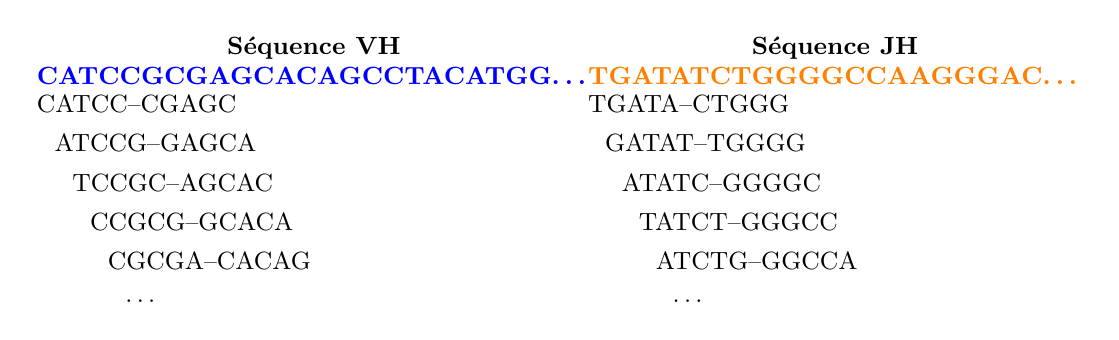
\begin{tikzpicture}[node distance=0cm, thick, font=\small]

    % Séquence VH
    \node[anchor=west] (VH) at (0,0) 
    {\shortstack{\textbf{Séquence VH} \\ \textbf{\textcolor{blue}{CATCCGCGAGCACAGCCTACATGG\dots}}}};
    
    % k-mer espacés séquence VH
    \foreach \i [count=\j from 0] in {
        CATCC--CGAGC,
        ATCCG--GAGCA,
        TCCGC--AGCAC,
        CCGCG--GCACA,
        CGCGA--CACAG,
        \dots
    } {
        \pgfmathsetmacro\xshift{\j*0.225}
        \pgfmathsetmacro\ypos{-0.5*(\j+1.1)}
        \node[anchor=west] at (\xshift,\ypos) {\i};
    }

    % Séquence JH
    \node[anchor=west] (J) at (7,0)
    {\shortstack{\textbf{Séquence JH} \\ \textbf{\textcolor{orange}{TGATATCTGGGGCCAAGGGAC\dots}}}};

    % k-mer espacés séquence JH
    \foreach \i [count=\j from 0] in {
        TGATA--CTGGG,
        GATAT--TGGGG,
        ATATC--GGGGC,
        TATCT--GGGCC,
        ATCTG--GGCCA,
        \dots
    } {
        \pgfmathsetmacro\xshift{7 + \j*0.215}
        \pgfmathsetmacro\ypos{-0.5*(\j+1.1)}
        \node[anchor=west] at (\xshift,\ypos) {\i};
    }

    \end{tikzpicture}
    \caption{Génération de l'index à partir de \textit{k-mer} des séquences germinales 
    \textcolor{blue}{VH (à gauche)} et \textcolor{orange}{JH (à droite)}.}
    \label{fig:index}
\end{figure}

    
La seconde étape consiste à traverser l'ensemble des \textit{reads} en recherchant des fenêtres $\mathbf{w}$ qui recouvrent 
la région \gls{cdr}3 par comparaison de chacun des \textit{k-mer} du \textit{read} à ceux des index générés. Brièvement cette 
approche consiste à conserver les \textit{reads} qui contiennent les \textit{k-mer} d'une séquence V et ceux d'une séquence J, 
de façon à former une fenêtre $\mathbf{w}$ débutant par les derniers \textit{k-mer} de la séquence V et se terminant 
par les premiers \textit{k-mer} de la séquence J (\autoref{fig:vidjil-algo}).
Cette approche permet une détection rapide (qui croit linéairement avec le nombre de nucléotides \footnote{En pratique l'étape de détection des fenêtres 
est de compléxité $O(ln)$ et plus récemment $O(l'n)$ où $l$ est le nombre de recombinaisons des systèmes, $l'$ le nombre moyen avec $l' \ll l$, et $n$ 
la taille de la séquence.}), robuste et efficace 
des séquences recombinées. Une fois les fenêtres détectées, \textit{vidjil-algo} regroupe les \textit{reads} en clones, 
puis procède à une segmentation et une annotation des séquences identifiées \footnote{Cette étape de désignation est elle de compléxité $O(Mn)$, et $O(M'n)$ à présent, 
$M$ désignant la taille totale des gènes considérés, et $M'$ un sous ensemble tel que $M' \ll M$.}. 

\begin{figure}[H]
    \centering
    \begin{tikzpicture}[node distance=0cm, thick, font=\small]

    % Première ligne
    \node[
        rectangle, 
        fill=blue!30, 
        text width=4cm, 
        align=left,
        minimum width=4cm, 
        minimum height=0.6cm
        ] at (0,0) (v_predicted1) {VVVVVV};

    \node[right=of v_predicted1] (sub) {\textcolor{red}{X}};

    \node[
        rectangle, 
        right=of sub, 
        fill=blue!30, 
        text width=3cm, 
        align=left,
        minimum width=3cm, 
        minimum height=0.6cm
        ] (v_predicted2) {VVVVVVVVVV};

    \node[
        rectangle, 
        right=2cm of v_predicted2, 
        fill=orange!30, 
        text width=5cm, 
        align=left,
        minimum width=5cm, 
        minimum height=0.6cm
        ] (j_predicted) {JJJJJJJJJJJJJJJJJJ};

    % Fenêtre w
    \draw[draw=violet, thick]
        ($(v_predicted2.west)!0.5!(v_predicted2.east) + (0,0.35)$) rectangle
        ($(j_predicted.west)!0.5!(j_predicted.east) + (0,-0.35)$);

    % Annotations
    \node[anchor=north west] at ([yshift=-1pt]v_predicted1.south west) 
        {\scriptsize \textbf{\textcolor{blue}{V prédit}}};

    \draw[thick, blue] ($(v_predicted1.west)+(0,-0.8)$) -- ($(v_predicted2.east)+(0,-0.8)$) 
        node[anchor=north west] at ([yshift=-0.5cm]v_predicted1.south west) 
        {\scriptsize \textcolor{blue}{V réel}};

    \node[anchor=north east] at ([yshift=-1pt]j_predicted.south east) 
        {\scriptsize \textbf{\textcolor{orange}{J prédit}}};

    \draw[thick, orange] ($(j_predicted.west)+(0,-0.8)$) -- ($(j_predicted.east)+(0,-0.8)$) 
        node[anchor=north east] at ([yshift=-0.5cm]j_predicted.south east) 
        {\scriptsize \textcolor{orange}{J réel}};
        
    \node[above=3pt of sub] {\scriptsize \textbf{\textcolor{red}{Substitution}}};

    \node at ($(v_predicted2)!0.5!(j_predicted)+(0,0.6)$) {\scriptsize \textbf{\textcolor{violet}{Fenêtre extraite w}}};

    % Deuxième ligne
    \begin{scope}[yshift=-2cm]

    \node[
        rectangle, 
        fill=blue!30, 
        text width=4cm, 
        align=left,
        minimum width=4cm, 
        minimum height=0.6cm
        ] at (0,0) (v_predicted1b) {VVVVVVVVVVVV};

    \node[
        rectangle, 
        right=-0.5 cm of v_predicted1b, 
        fill=blue!30,
        minimum width=2.5cm, 
        minimum height=0.6cm
        ] (v_predicted2b) {};

    \node[right=of v_predicted2b] (subb) {\textcolor{red}{X}};

    \node[
        rectangle, 
        right=3.7cm of v_predicted2b, 
        fill=orange!30, 
        text width=5cm, 
        align=left,
        minimum width=5cm, 
        minimum height=0.6cm
        ] (j_predictedb) {JJJJJJJJJJJJJJJJJJ};

    % Fenêtre w
    \draw[draw=violet, thick]
        ($(v_predicted2b.west)!0.5!(v_predicted2b.east) + (0,0.35)$) rectangle
        ($(j_predictedb.west)!0.4!(j_predictedb.east) + (0,-0.35)$);

    % Annotations
    \node[anchor=north west] at ([yshift=-1pt]v_predicted1b.south west) 
        {\scriptsize \textbf{\textcolor{blue}{V prédit}}};

    \draw[thick, blue] ($(v_predicted1b.west)+(0,-0.8)$) -- ($(v_predicted2b.east)+(1.7,-0.8)$) 
        node[anchor=north west] at ([yshift=-0.5cm]v_predicted1b.south west) 
        {\scriptsize \textcolor{blue}{V réel}};

    \node[anchor=north east] at ([yshift=-1pt]j_predictedb.south east) 
        {\scriptsize \textbf{\textcolor{orange}{J prédit}}};

    \draw[thick, orange] ($(j_predictedb.west)+(0,-0.8)$) -- ($(j_predictedb.east)+(0,-0.8)$) 
        node[anchor=north east] at ([yshift=-0.5cm]j_predictedb.south east) 
        {\scriptsize \textcolor{orange}{J réel}};
        
    \node[above=3pt of subb] {\scriptsize \textbf{\textcolor{red}{Substitution}}};

    \node at ($(v_predicted2b)!0.7!(j_predictedb)+(0,0.6)$) {\scriptsize \textbf{\textcolor{violet}{Fenêtre extraite w}}};

    \end{scope}

    \end{tikzpicture}
    \caption{Illustration du fonctionnement de \textit{vidjil-algo} sur deux lectures successives.}
    \label{fig:vidjil-algo}
\end{figure}

% JavaScript Object Notation (JSON) :o je ne connaissais même pas l'acronyme !
Les résultats ainsi générés par \textit{vidjil-algo} sont rassemblés dans un fichier \textit{.vidjil} au format \gls{json} où 
l'on retrouvera des métadonnées en lien avec l'échantillon analysé et un ensemble de données relatif à chaque clone 
identifié par \textit{vidjil-algo} (\autoref{lst:json-vidjil}).

\begin{figure}[H]
\begin{lstlisting}[language=json, 
caption={Extrait d'une sortie de \textit{vidjil-algo}.},
label={lst:json-vidjil}]
"clones": [
    {
        "_average_read_length": ["151.80"],
        "_coverage_info": [ "132 bp (86% of 151.8 bp)"],
        "germline": "IGH",
        "id": "GGGGATAAATTACGATTTTTGGAGTGGTTATTAT...GGGGGTT",
        "name": "IGHV1-8*01 0/CGGGGGGATAA/2 IGHD3-3*01 0/GGTATGGGGGGTTTTAG/7 IGHJ4*02",
        "reads": [498126],
        ...
    }
]
\end{lstlisting}
\end{figure}

En parallèle, \textit{Vidjil} désigne également l'application web \footnote{\url{https://app.vidjil.org/}} 
permettant de visualiser et de manipuler les résultats produits par \textit{vidjil-algo}. 
Elle prend aussi en charge la création et la gestion des comptes utilisateurs, des profils patients, etc. (\autoref{fig:vidjil-web}). 
L'application est développée côté serveur en \texttt{Python}, à l'aide du \textit{framework} \href{https://py4web.com}{\texttt{py4web}} 
(anciennement \texttt{web2py}), et côté client en \texttt{JavaScript}. La base de données utilisée est \texttt{MySQL}, 
le tout étant orchestré via le déploiement de conteneurs \texttt{Docker}.

\begin{figure}[H]
    \centering
    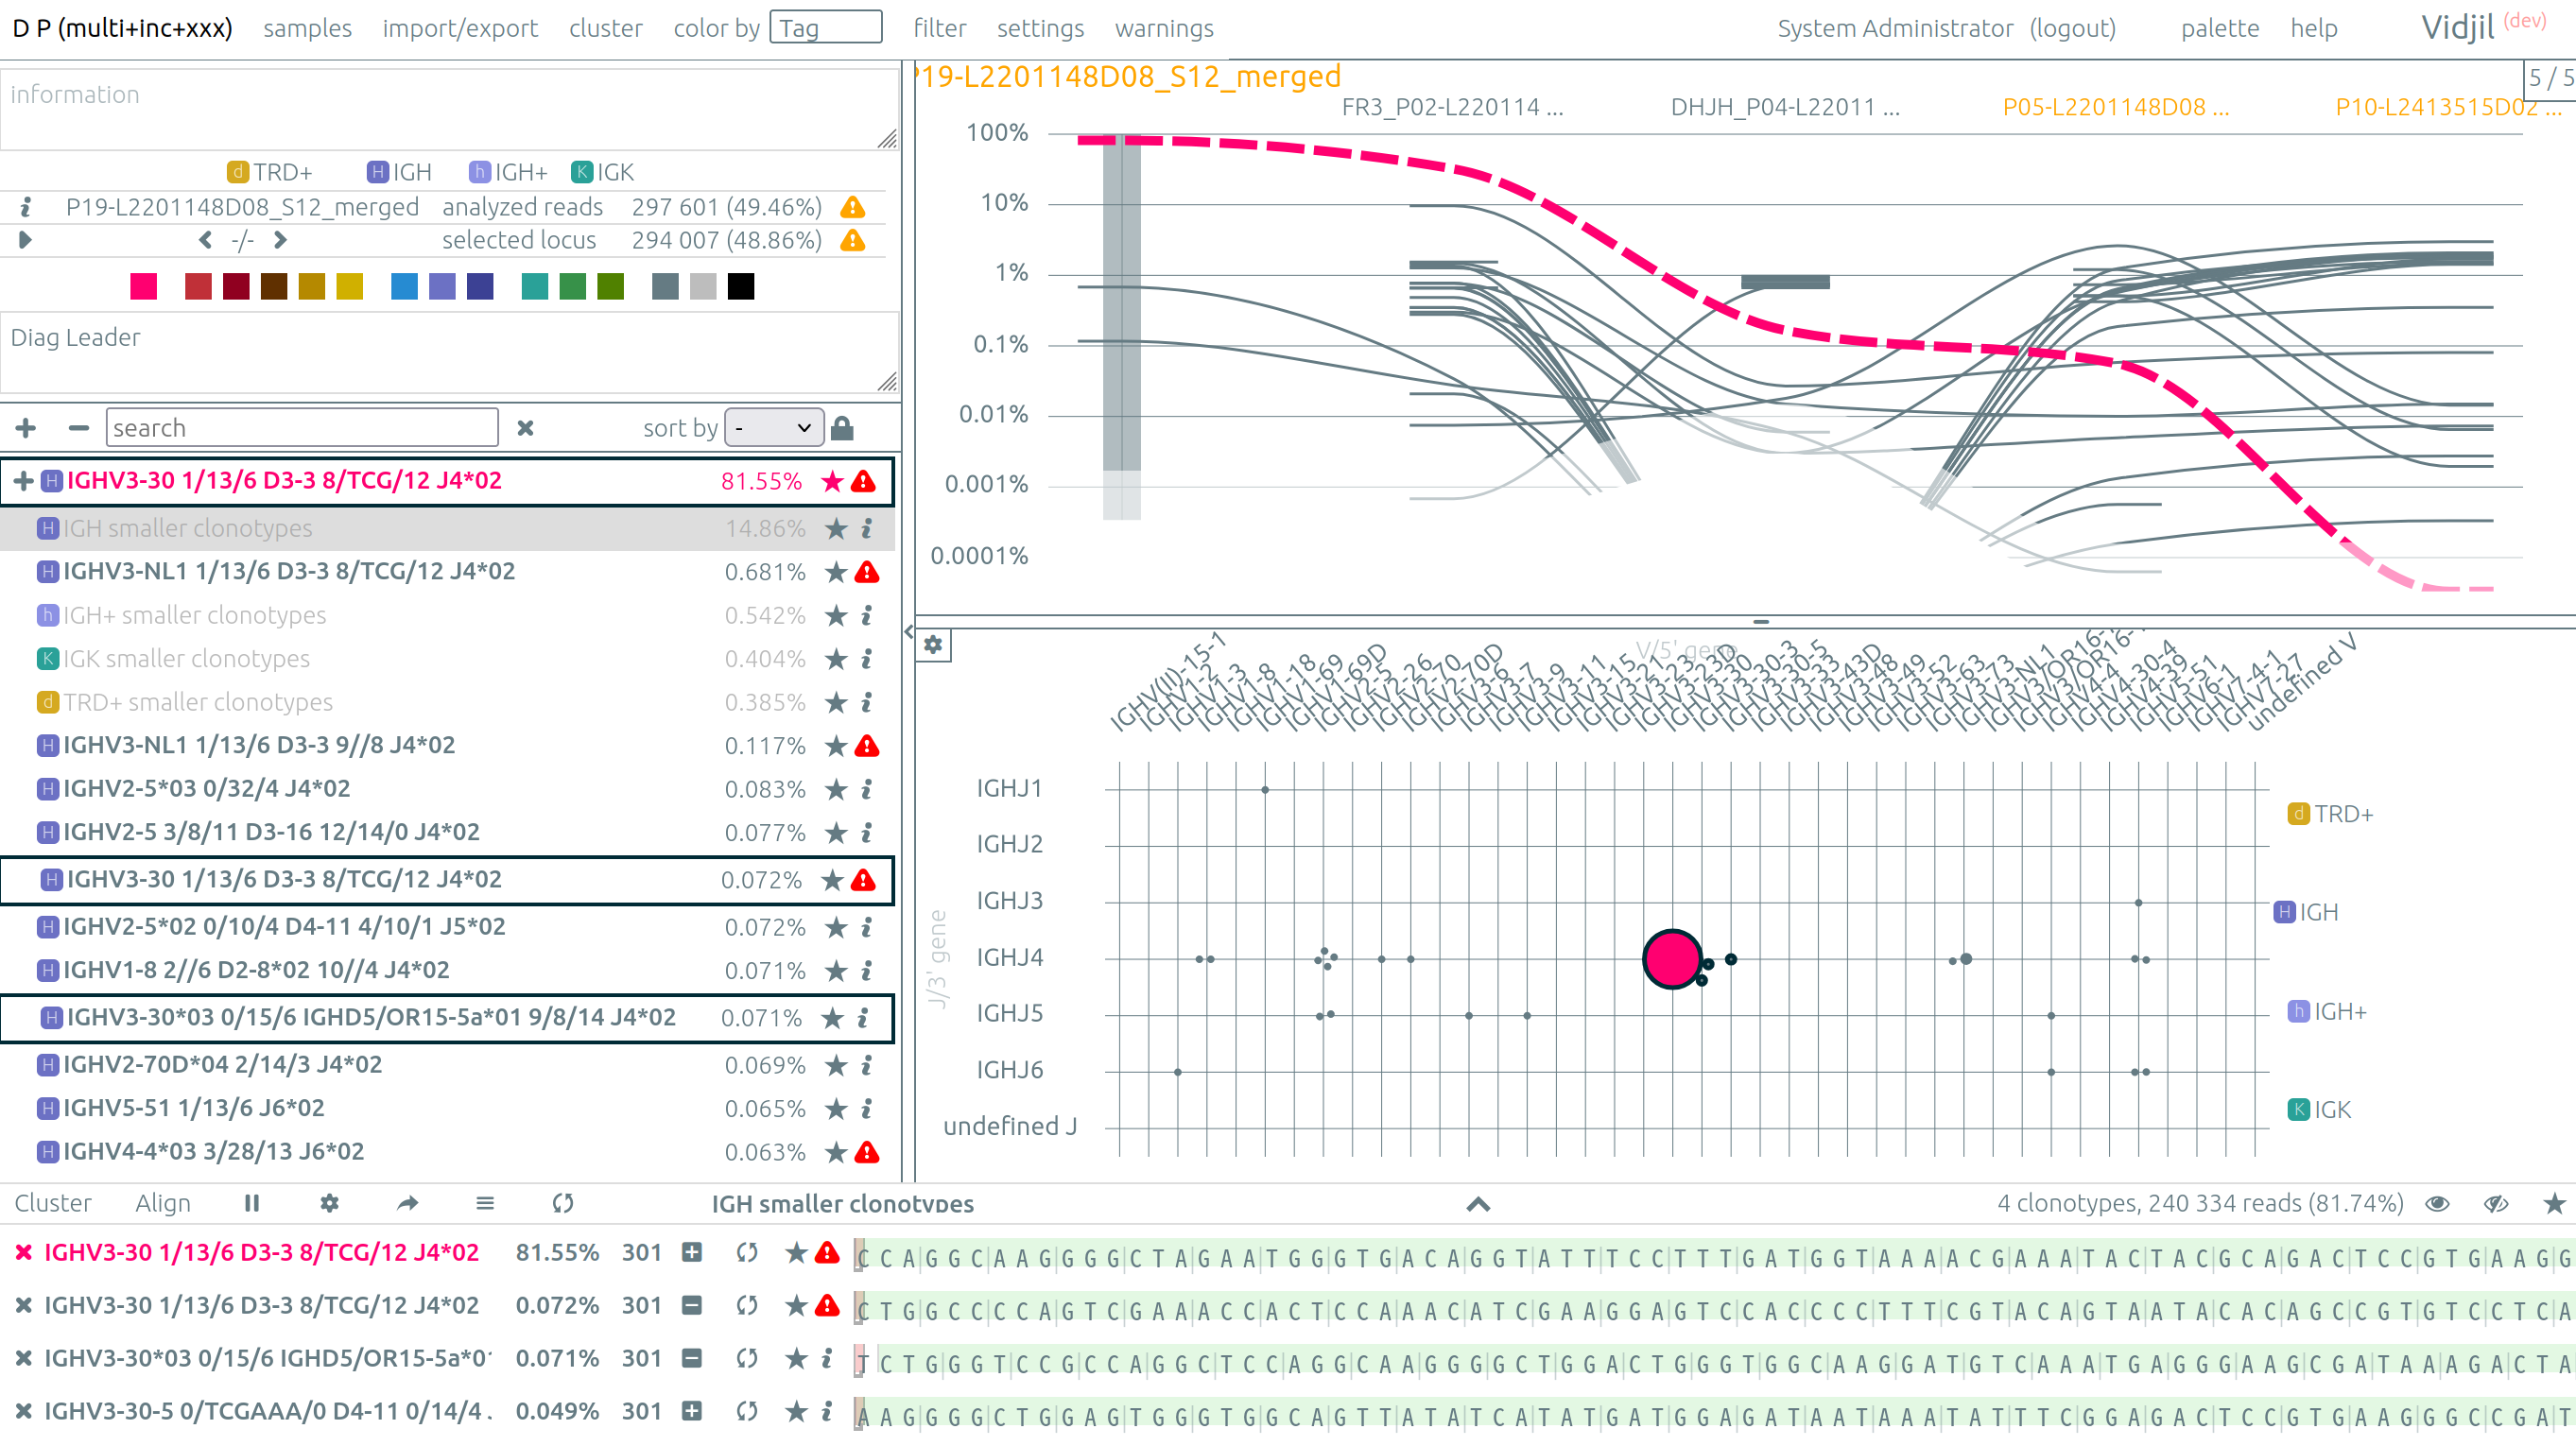
\includegraphics[width=1\textwidth]{images/vidjil-web.png}
    \caption{Interface de la plateforme web \textit{Vidjil}. 
    Liste des clones identifiés à gauche, visualisation de la cinétique des clones en haut à gauche, 
    familles \gls{vdj} en bas à droite, et séquences des clones sélectionnés en bas.}
    \label{fig:vidjil-web}
\end{figure}

\section{Applications en oncohématologie}

L'analyse du répertoire des gènes \gls{vdj} est particulièrement utile en oncohématologie, 
où la quasi unicité de chaque réarrangement \gls{vdj} peut servir de marqueur clonal hautement 
spécifique de certaines cellules tumorales et ainsi permettre leur détection et leur suivi \cite{hultcrantzBaselineVDJClonotype2020}.

\vspace{1em}
% Alors je pense qu'on ne met pas de s quand on utilise les acronyme LAM LAL
Avant toute chose, il peut être utile de dresser un panorama rapide des hémopathies malignes afin de 
mieux comprendre l'importance de l'analyse du répertoire des gènes \gls{vdj} dans ces situations.  
Ces pathologies regroupent ce qu'on appelle communément les « cancers du sang » et peuvent se séparer selon
leur origine en quatre grandes catégories. Une première séparation peut être établie entre les hémopathies 
myéloïdes et lymphoïdes selon l'origine des cellules. Brièvement, les cellules du sang et de la moelle sont soit de 
lignée lymphoïde pour les lymphocytes (B, T, NK et autres non conventionnels) et précurseurs, soit de lignée myéloïde 
pour le reste des cellules (hématies, plaquettes, polynucléaires, monocytes) et leurs précurseurs. Une seconde séparation 
est établie selon la maturité des cellules : on parle alors de \glspl{lam} et de \glspl{lal} lorsque la cellule 
tumorale dérive d'un précurseur, et de \glspl{smp} et de \glspl{slp}/\glspl{lnh} lorsque la cellule est mature (\autoref{fig:hemopathies}) 
\cite{alaggio5thEditionWorld2022a, khoury5thEditionWorld2022}.

% C'et quoi cette horreur ???? (je parle du graphique) Je sais qu'on aime la
% cyto mais non ; je ferme les yeux j'ai les diapos de claude écriture jaune
% fond bleu marine-noire
% iconographie plus simple et carré comme celle là :
% https://gramproject.com/wp-content/uploads/2020/08/Haematology-cell-lineages-and-malignancies.png
% On la modifie légèrement pour ajouter MDS comme ça on a un un truc complet 
% Et en plus tu introduit le MM avec ce style de graph plus facilement 

\begin{figure}[H]
    \centering
    \begin{tikzpicture}[scale=1, every node/.style={font=\small}]

    \filldraw[fill=violet!30, opacity=0.2] (-2.5,0) rectangle (3,4); 
    \filldraw[fill=violet!60, opacity=0.4] (-2.5,-4) rectangle (3,0); 
    \filldraw[fill=blue!30, opacity=0.2] (3,0) rectangle (8.5,4); 
    \filldraw[fill=blue!60, opacity=0.4] (3,-4) rectangle (8.5,0);

    \node[rotate=90] at (-3,2) {Précurseurs (immature)};
    \node[rotate=90] at (-3,-2) {Cellules matures};
    \node at (0,4.3) {Myéloïde};
    \node at (6,4.3) {Lymphoïde};

    \node at (0,3.5) {\small \textbf{\gls{lam}}};
    \node at (6,3.5) {\small \textbf{\gls{lal}}};
    \node at (0,-0.5) {\small \textbf{\gls{smp}}};
    \node at (4.7,-0.5) {\small \textbf{\gls{slp}}};
    \node at (7,-0.5) {\small \textbf{\gls{lnh}}};

    \node at (0,1.7) {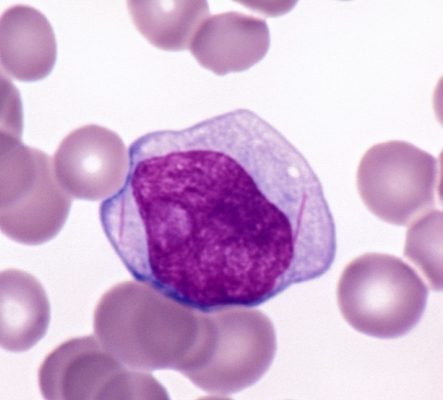
\includegraphics[width=3cm]{images/lam.jpg}};
    \node at (6,1.7) {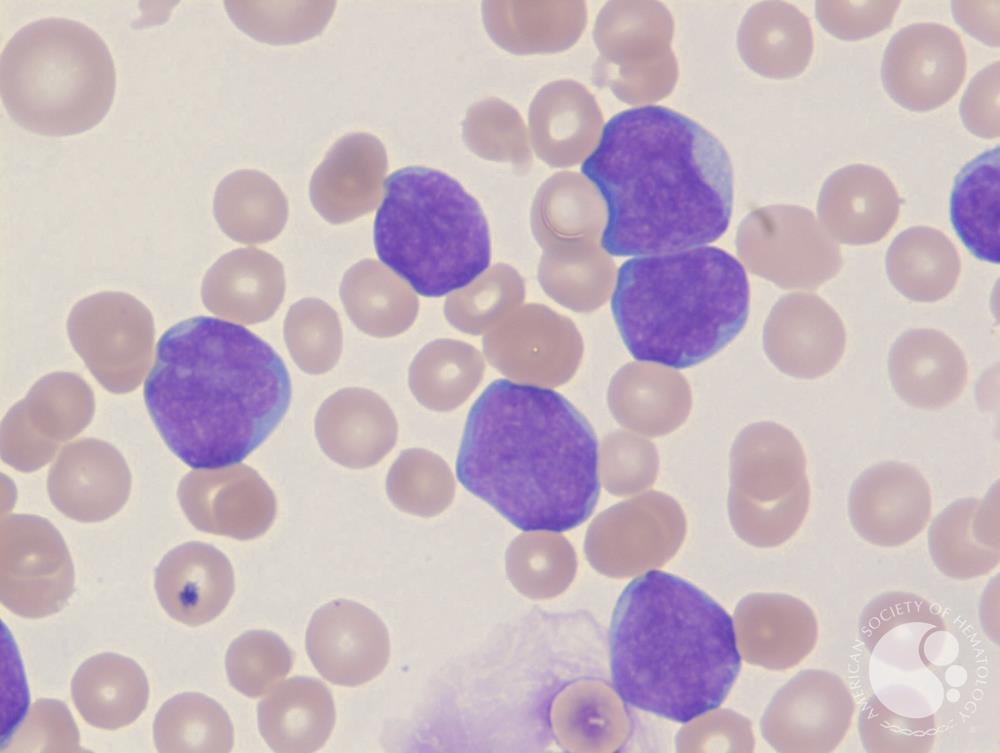
\includegraphics[width=3cm]{images/lal.jpeg}};
    \node at (-1,-2) {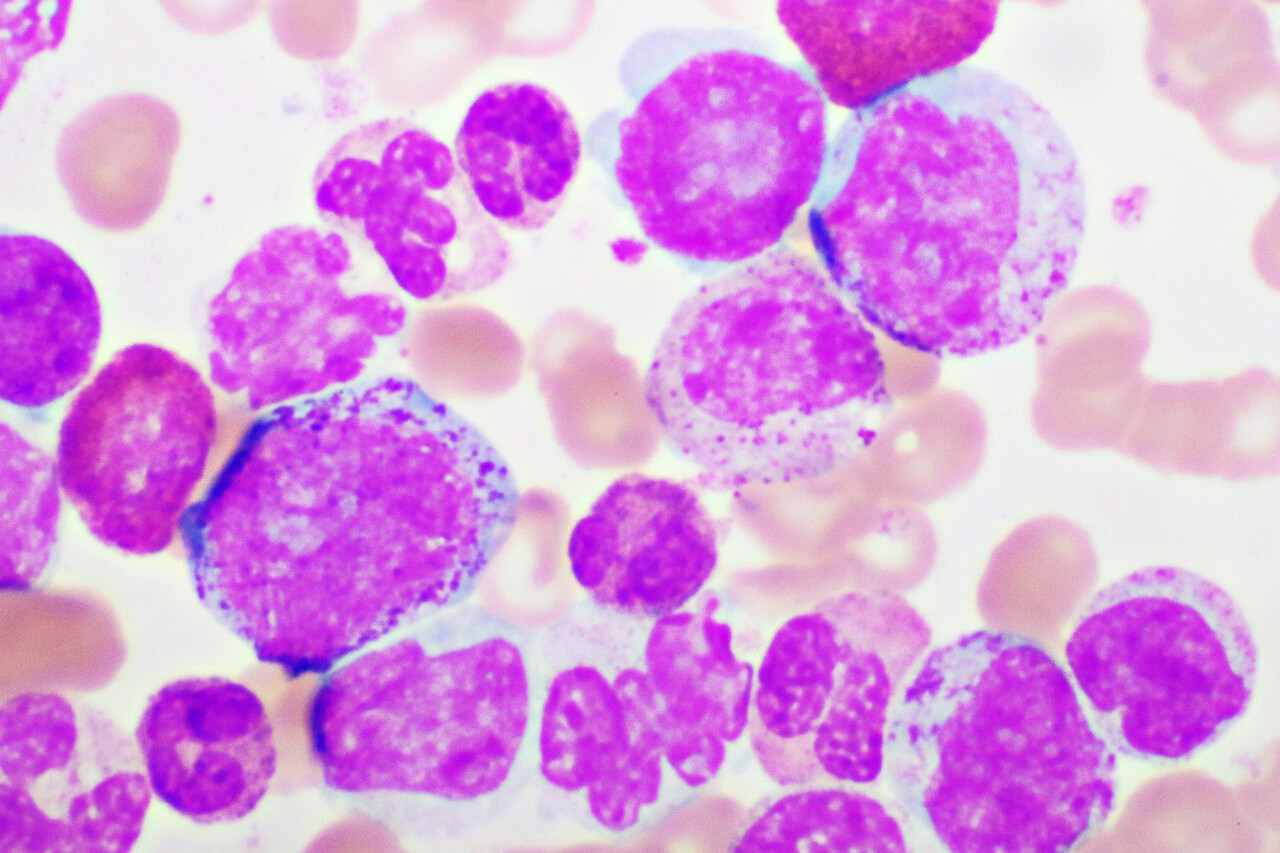
\includegraphics[width=2cm]{images/lmc.jpg}};
    \node at (1.2,-3) {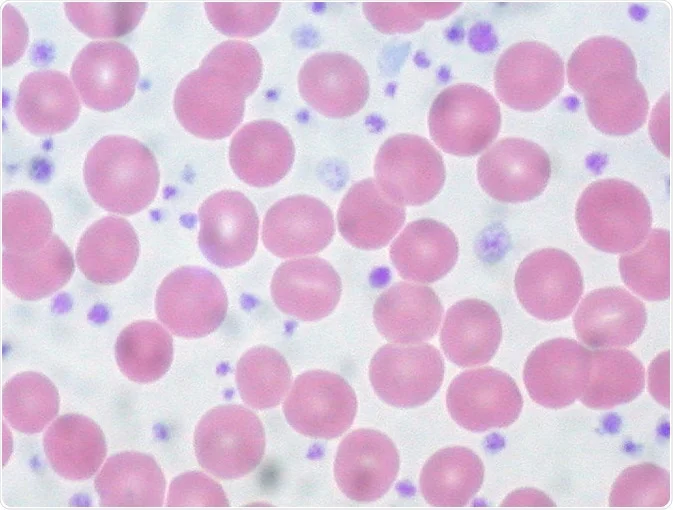
\includegraphics[width=2cm]{images/te.png}};
    \node at (4.7,-2) {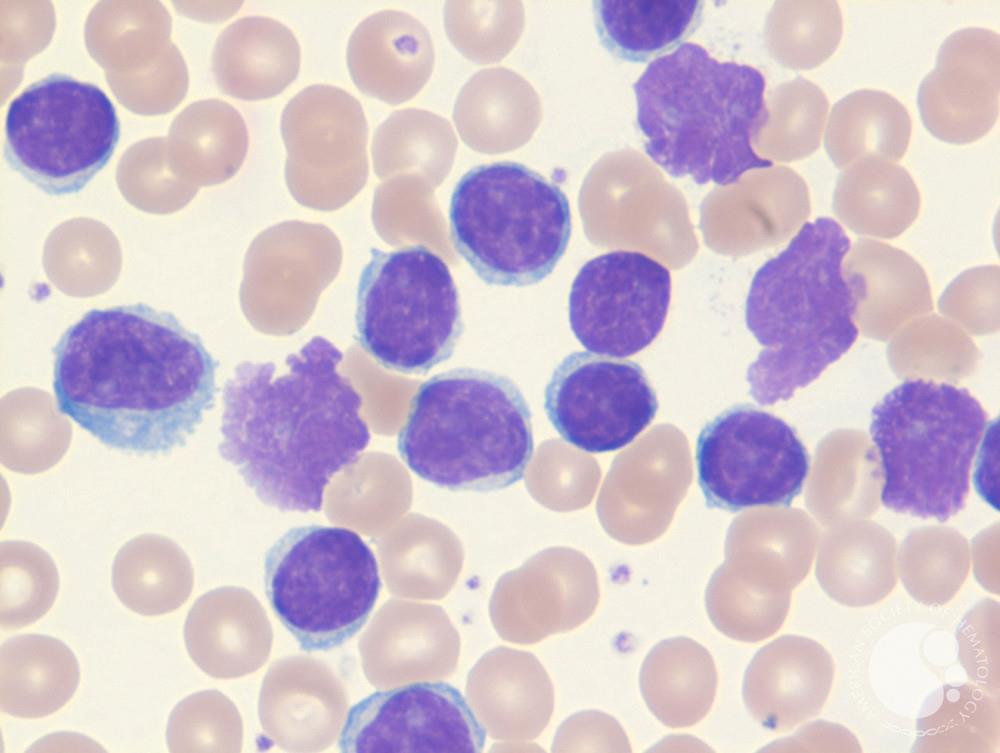
\includegraphics[width=2cm]{images/llc.jpeg}};
    \node at (7, -3) {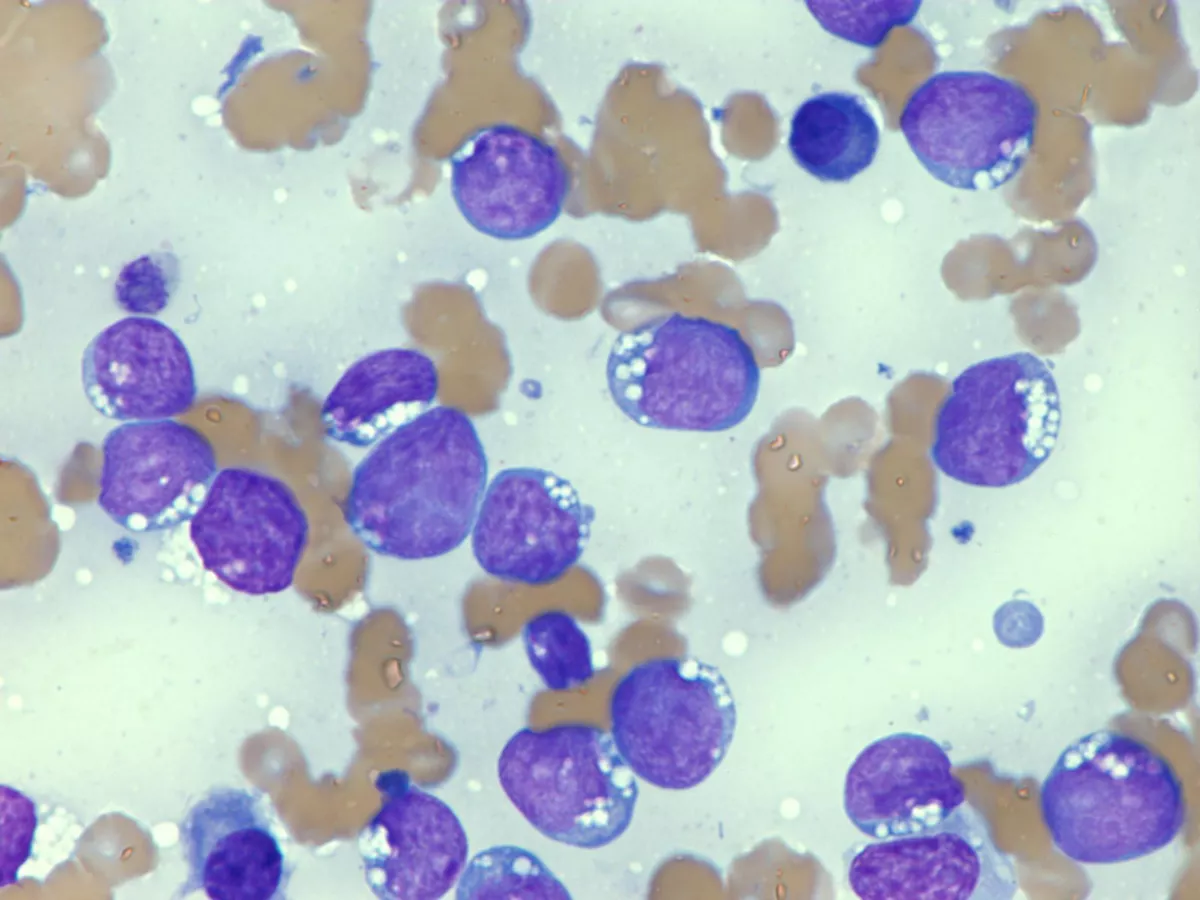
\includegraphics[width=2cm]{images/burkitt.png}};

    \draw[thick] (3,4.5) -- (3,-4.5); 
    \draw[thick] (-3,-0) -- (9,-0); 

    \end{tikzpicture}
    \caption{Classification des hémopathies malignes selon la lignée (myéloïde vs lymphoïde) 
    et le degré de maturité cellulaire (précurseur vs mature).}
    \label{fig:hemopathies}
\end{figure}


Dès lors \textit{Vidjil} trouve son utilité dans les hémopathies lymphoïdes, principalement dans les \glspl{lal} et les 
\glspl{llc} où il permet l'identification des réarrangements \gls{vdj} des \glspl{ig} et des \glspl{tcr} à des fins diverses.
Par exemple, dans les \glspl{llc} il permet d'identifier et d'annoter le segment V du réarrangement \textit{\gls{igh}} du clone tumoral, pour 
ensuite étudier le taux de mutations face aux séquences germinales, servant de marqueur pronostique fort de la pathologie
\cite{crombieIGHVMutationalStatus2017}.

\vspace{1em}

Dans le cadre de ce travail, nous nous sommes intéressés à une pathologie en particulier : le \gls{mm}, que l'on peut rattacher
au groupe des hémopathies lymphoïdes matures. Cette pathologie se caractérise par une prolifération maligne de plasmocytes, cellules
dérivées des lymphocytes B, responsables de la production et de la sécrétion des \glspl{ig} (anticorps) \cite{briglePathobiologyDiagnosisMultiple2017}. 
Elles constituent le stade le plus mature de la lymphopoïèse B, à la suite de la différenciation des lymphocytes B naïfs 
au contact de l'antigène, et sont les principaux acteurs de la réponse immunitaire humorale adaptative.

\vspace{1em}

Dans le \gls{mm}, les plasmocytes malins prolifèrent de manière incontrôlée, entraînant une altération du fonctionnement normal de la moelle osseuse,
avec des anémies, un déficit immunitaire secondaire, des atteintes osseuses, et une insuffisance rénale. Une partie de ces symptômes est causée
par la production d'une \gls{ig} monoclonale, dont la détection par électrophorèse constitue un élément diagnostique majeur, au même titre que la
prolifération médullaire des plasmocytes malins et les autres signes cliniques et biologiques précédemment décrits \cite{cowanDiagnosisManagementMultiple2022a} 
(\autoref{fig:mm-cells-ig}).

\begin{figure}[H]
    \begin{minipage}{0.45\textwidth}
        \centering
        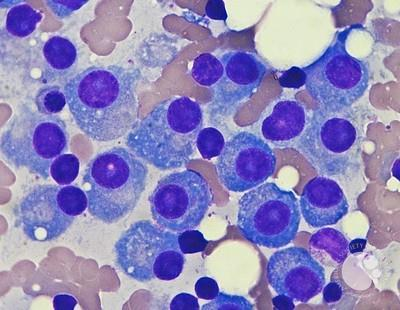
\includegraphics[width=1\textwidth]{images/mm_cells.jpeg}
    \end{minipage}
    \hfill
    \begin{minipage}{0.45\textwidth}
        \centering
        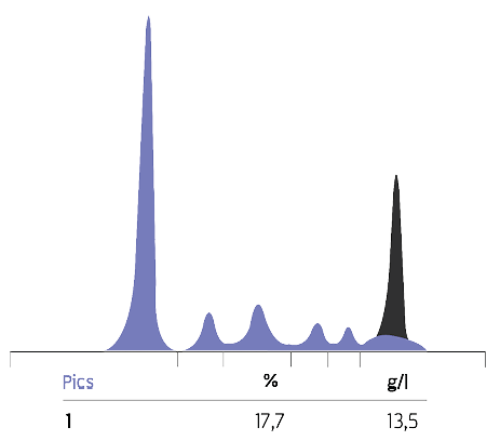
\includegraphics[width=01\textwidth]{images/pic.png}
    \end{minipage}
    \caption{Gauche : Prolifération de plasmocytes malins dans la moelle osseuse. 
    Droite : Electrophorèse des protéines sériques montrant la présence d'une \gls{ig} monoclonale (pic noir) 
    superposée à un profil normal en bleu.}
    \label{fig:mm-cells-ig}
\end{figure}

Le myélome multiple touche majoritairement les personnes âgées, avec un âge médian au diagnostic d'environ 70 ans. Il représente environ 10 \%
des hémopathies malignes et près de 1 \% de l'ensemble des cancers. En France, on estime à environ 6 000 le nombre de nouveaux cas chaque année 
\cite{spfSurviePersonnesAtteintes}.

\vspace{1em}

Sur le plan thérapeutique, les stratégies ont considérablement évolué ces dernières années. Le traitement repose sur une approche personnalisée
selon l'âge et l'état général du patient. Chez les patients éligibles, une chimiothérapie d'induction est souvent suivie d'une autogreffe de cellules
souches hématopoïétiques. Chez les patients plus âgés ou fragiles, des protocoles associant agents immunomodulateurs (tels que la lénalidomide),
inhibiteurs du protéasome (comme le bortézomib) et anticorps monoclonaux (notamment l'anti-CD38, daratumumab) sont privilégiés. Le traitement de
maintenance et la surveillance à long terme permettent de prolonger la réponse et de retarder les rechutes, fréquentes dans cette pathologie chronique 
\cite{cowanDiagnosisManagementMultiple2022a}.

\vspace{1em}

En ce qui concerne le \gls{mm}, l'intérêt de l'analyse du répertoire \gls{vdj} se rapproche de celui des \glspl{lal} où l'identification 
de réarrangement \gls{vdj} (en l'occurrence ici des \textit{\gls{igh}} ou des \textit{\gls{igk}} et \textit{\gls{igl}}) sert de marqueur unique (dit de clonalité) 
de la cellule tumorale, et permet ainsi de suivre l'évolution de la maladie.

\section{Maladie résiduelle et ADN circulant tumoral}

Comme de nombreuses autres hémopathies, le \gls{mm} est une pathologie dont l'évolution clinique peut être très hétérogène. 
Si certaines caractéristiques observées au diagnostic permettent de dresser un pronostic plus ou moins favorable, 
la trajectoire de la maladie reste souvent difficile à prédire \cite{hanamuraMultipleMyelomaHighrisk2022}. 
Dans ce contexte, un marqueur particulièrement pertinent de l'évolution de la maladie et de la réponse au traitement 
est la présence d'une \gls{mrd} dite indétectable.

\vspace{1em}

La \gls{mrd} désigne la persistance de cellules tumorales résiduelles non détectables 
par les méthodes conventionnelles (telles que l'analyse morphologique ou biochimique), mais que l'on peut mettre en évidence 
grâce à des techniques de haute sensibilité, comme la \gls{cmf} multiparamétrique ou la biologie moléculaire. Elle représentent 
en quelque sorte la « face cachée de l'iceberg » de la maladie, qui persiste même lorsque les signes cliniques et biologiques 
ont disparu (\autoref{fig:mrd-techniques}).
Dans le cas spécifique du \gls{mm}, l'évaluation de la \gls{mrd} repose souvent sur la détection de cellules présentant des 
aberrations phénotypiques par \gls{cmf} ou sur la détection de réarrangements \gls{vdj} propres au clone tumoral, permettant un suivi très ciblé 
mais plus complexe à mettre en oeuvre \cite{bertaminiMRDAssessmentMultiple2021}.

\begin{figure}[H]
    \centering
    \begin{tikzpicture}

    % iceberg
    \node at (0,0.8) {
\includegraphics[width=10cm]{images/iceberg.jpg}}; 

    % seuils
    \draw[dashed] (-3.5,2.5) -- (3.5,2.5);
    \draw[dashed] (-3.5,-0.5) -- (3.5,-0.5);
    \draw[dashed] (-3.5,-2) -- (3.5,-2);

    \node at (0,3.2) {\textbf{Maladie à expression clinique}};
    \node at (0,0.8) {\textbf{\gls{mrd}}};
    \node at (0,-1.4) {\textbf{\gls{mrd} non quantifiable}};
    \node at (0,-3) {\textbf{Maladie non détectable}};

    % axe cellules leucémiques 
    \draw[very thick] (-3.5,4.2) -- (-3.5,-4.2);
    \node[rotate=90] at (-4.5,0) {Nombre de cellules leucémiques};

    \node at (-3.9,4.0) {$10^{12}$};
    \node at (-3.9,2.5) {$10^{10}$};
    \node at (-3.9,1) {$10^{8}$};
    \node at (-3.9,-0.5) {$10^{6}$};
    \node at (-3.9,-2) {$10^{4}$};
    \node at (-3.9,-3.5) {$10^{2}$};

    % axe valeurs de mrd
    \draw[very thick] (3.5,4.2) -- (3.5,-4.2);
    \node[rotate=-90] at (4.7,0) {Valeurs de \gls{mrd}};

    \node at (4,2.5) {$10^{-2}$};
    \node at (4,1) {$10^{-4}$};
    \node at (4,-0.5) {$10^{-6}$};
    \node at (4,-2) {$10^{-8}$};
    \node at (4,-3.5) {$10^{-10}$};

    % Techniques de détection
    \node[align=center, text width=4cm, font=\bfseries] at (7,4.4) {Méthodes de mesure};

    \node[anchor=west] at (5.5,3.3) {
\includegraphics[width=1.5cm]{images/microscope.png}};
    \node[anchor=west] at (7.8,3.3) {Microscopie optique};

    \node[anchor=west] at (5.5,1.5) {
\includegraphics[width=1.5cm]{images/cmf.png}};
    \node[anchor=west] at (7.8,1.5) {\gls{cmf}};

    \node[anchor=west] at (5,0) {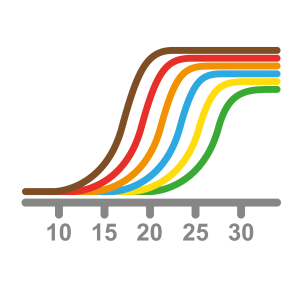
\includegraphics[width=1.5cm]{images/pcr.png}};
    \node[anchor=west] at (7.8,0) {\gls{pcr} quantitative};

    \node[anchor=west] at (6.2,-0.5) {
\includegraphics[width=1.5cm]{images/ngs.png}};
    \node[anchor=west] at (7.8,-0.5) {\gls{hts}};

    \node[align=center] at (7.5,-2.5) {\gls{mrd} non détectable \\ avec les méthodes actuelles};
    \node[align=center] at (7.5,-3.5) {\textbf{Guérison}};

    \end{tikzpicture}
    \caption{
    Représentation schématique des techniques de détection de la \gls{mrd} et des seuils de détection en 
    regard du nombre de cellules leucémiques.
    Les techniques de détection sont classées selon leur sensibilité, allant de la morphologie à la biologie 
    moléculaire. Adapté de \citeauthor{sayginMeasurableResidualDisease2022} \cite{sayginMeasurableResidualDisease2022}.
    }
    \label{fig:mrd-techniques}
\end{figure}



L'intérêt pronostique de la \gls{mrd} a largement été démontré dans d'autres hémopathies malignes, notamment dans les \gls{lal} et \gls{lam}, 
où elle s'est imposée comme un outil essentiel pour guider et adapter les stratégies thérapeutiques. Dans le \gls{mm}, l'absence de \gls{mrd} 
après traitement est également associée à une durée de rémission prolongée et à une survie globale améliorée. A l'inverse, une \gls{mrd} détectable, 
même à très faible niveau, constitue un facteur de risque important de rechute précoce (\autoref{fig:mrd})
\cite{munshiLargeMetaanalysisEstablishes2020}.

\vspace{1em}

Ainsi, le suivi de la \gls{mrd} tend aujourd'hui à devenir non seulement un critère d'évaluation de l'efficacité thérapeutique, mais aussi un objectif 
thérapeutique propre dans le \gls{mm}. De plus en plus d'essais cliniques intègrent désormais la \gls{mrd} comme critère principal d'évaluation, 
voire comme élément décisionnel pour intensifier, adapter ou interrompre un traitement.

\begin{figure}[H]
    \centering
    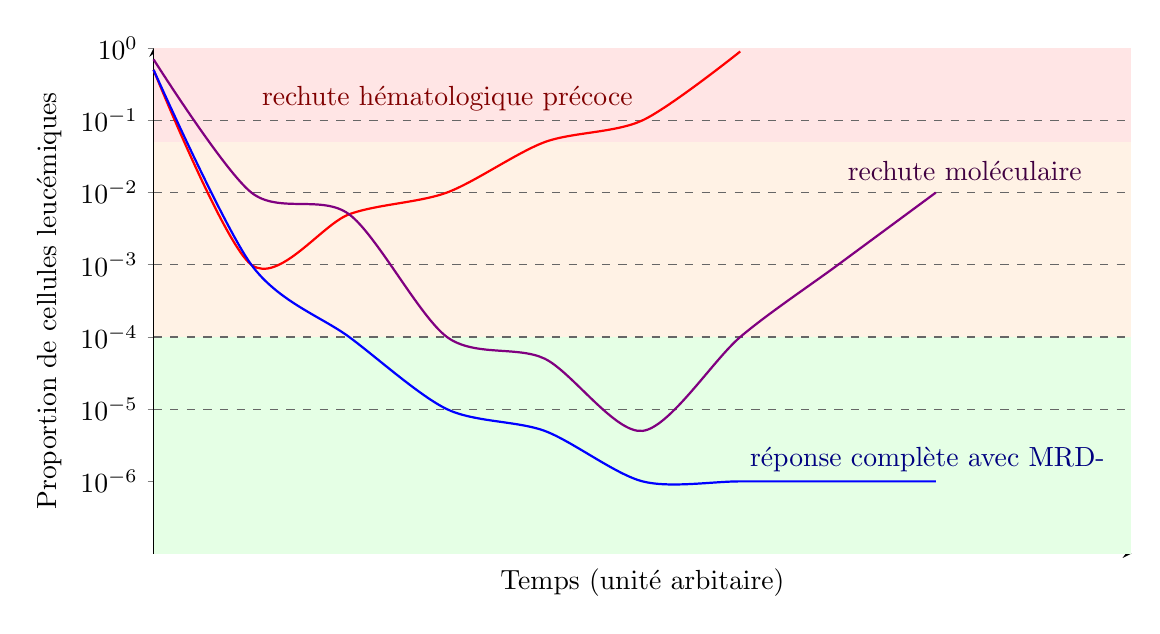
\begin{tikzpicture}
    \begin{semilogyaxis}[
        width=14cm,
        height=8cm,
        xlabel={Temps (unité arbitaire)},
        ylabel={Proportion de cellules leucémiques},
        ymin=1e-7, ymax=1,
        ytick={1e0,1e-1,1e-2,1e-3,1e-4,1e-5,1e-6},
        yticklabels={$10^{0}$,$10^{-1}$,$10^{-2}$,$10^{-3}$,$10^{-4}$,$10^{-5}$,$10^{-6}$},
        xtick=\empty,
        axis lines=left,
        grid=none,
        clip=false,
    ]

    % sections d'arrière plan
    \addplot [draw=none, fill=red!10]
     coordinates {
        (0,1e0) (10,1e0) (10,5e-2) (0,5e-2)
    } -- cycle;

    \addplot [draw=none, fill=orange!10
    ] coordinates {
        (0,5e-2) (10,5e-2) (10,1e-4) (0,1e-4)
    } -- cycle;

    \addplot [draw=none, fill=green!10
    ] coordinates {
        (0,1e-4) (10,1e-4) (10,1e-7) (0,1e-7)
    } -- cycle;

    % lignes horizontales pour les seuils
    \foreach \y in {1e-1,1e-2,1e-3,1e-4,1e-5} {
        \addplot[dashed, color=black!60] coordinates {(0,\y) (10,\y)};
    }

    % réponse complète avec MRD-
    \addplot[thick, red, smooth] coordinates {
        (0,5e-1) (1,1e-3) (2,5e-3) (3,1e-2) (4,5e-2) (5,1e-1) (6,9e-1)
    };

    % rechute précoce
    \addplot[thick, blue, smooth] coordinates {
        (0,5e-1) (1,1e-3) (2,1e-4) (3,1e-5) (4,5e-6) (5,1e-6) (6,1e-6) (7,1e-6) (8,1e-6)
    };

    % rechute moléculaire 
    \addplot[thick, violet, smooth] coordinates {
        (0,7e-1) (1,1e-2) (2,5e-3) (3,1e-4) (4,5e-5) (5,5e-6) (6,1e-4) (7,1e-3) (8,1e-2)
    };

    % labels
    \node[align=left, anchor=west, blue!50!black] at (axis cs:6,2e-6) {réponse complète avec MRD-};
    \node[align=left, anchor=west, violet!50!black] at (axis cs:7,2e-2) {rechute moléculaire};
    \node[align=center, anchor=south east, red!50!black] at (axis cs:5,1e-1) {rechute hématologique précoce};

    \end{semilogyaxis}
    \end{tikzpicture}
    \caption{Suivi de la \gls{mrd} dans le temps. Exemple de trois réponses différentes selon le statut 
    de la \gls{mrd} : \textcolor{blue}{réponse complète avec \gls{mrd}- en bleu},  
    \textcolor{red}{rechute précoce en rouge} et \textcolor{violet}{rechute moléculaire en violet}.}
    \label{fig:mrd}
\end{figure}


Pour autant, l'analyse de la \gls{mrd} pose certaines difficultés, notamment en ce qui concerne la sensibilité et la spécificité des techniques utilisées.
Il faut pouvoir être en mesure de détecter un nombre extrêmement faible de cellules tumorales parmi une population très majoritaire de cellules normales,
ce qui exige des méthodes à très haut pouvoir résolutif et des échantillons de qualité et quantité suffisante.

\vspace{1em}

La \gls{cmf}, bien qu'accessible dans de nombreux centres, dépend fortement de l'expertise technique et de la standardisation
des panels d'anticorps utilisés. De plus, son seuil de détection, généralement de l'ordre de $10^{-3}$ à $5.10^{-5}$, peut s'avérer insuffisant dans certains contextes
thérapeutiques.

\vspace{1em}

Les approches moléculaires, comme le \gls{ngs} ciblant les réarrangements \gls{vdj}, offrent une sensibilité encore plus élevée (jusqu'à $10^{-6}$),
mais nécessitent une connaissance préalable du profil clonotypique du patient, ainsi qu'un accès à des plateformes technologiques spécialisées et solutions 
bioinformatiques dédiées. Par ailleurs, s'agissant du \gls{mm}, la détection des réarrangements \gls{vdj} peut être compliquée par la présence de nombreuses 
mutations sur la région V des \glspl{ig} à la suite du phénomène d'hypermutation somatique, ce qui peut rendre difficile l'amplification des séquences.

\vspace{1em}

Enfin, la représentativité de l'échantillon, souvent issu d'une ponction médullaire unique, peut aussi poser problème en raison de la distribution hétérogène
des plasmocytes tumoraux dans la moelle osseuse. Cette variabilité peut conduire à une sous-estimation de la \gls{mrd} en cas de prélèvement non représentatif.
Par ailleurs, la nécessité de prélèvements médullaires peut également constituer un frein à l'évaluation répétée de la \gls{mrd}, du fait de leur caractère
invasif, et souvent inconfortable pour le patient.

\vspace{1em}

Dans ce contexte, l'analyse des acides nucléiques circulants, et en particulier de l'\gls{adnc}, suscite un intérêt croissant. Ces fragments d'ADN, libérés dans le sang 
par les cellules tumorales et normales en apoptose ou en nécrose, peuvent refléter de manière globale la charge tumorale et permettre une évaluation non 
invasive de la \gls{mrd} (\autoref{fig:ctdna}). Contrairement à la ponction médullaire, un simple prélèvement sanguin (ou « biopsie liquide ») permet de suivre plus facilement 
et plus fréquemment l'évolution de la maladie.

\vspace{1em}

Bien que cette approche soit largement démocratisée dans le domaine de l'oncologie solide, elle reste encore en cours de validation en oncohématologie et demeure,
pour le moment, marginale, avec quelques applications dans le cadre des \glspl{lnh}. Dans les autres pathologies, les défis techniques liés à la faible concentration des 
\gls{adnc} et à la faible taille des fragments ($\approx$ 150 pb), à l'hétérogénéité génétique des hémopathies malignes et à l'absence de biomarqueurs universels 
limitent encore son déploiement en routine clinique \cite{daoUsingCfDNACtDNA2023}.

\begin{figure}[H]
    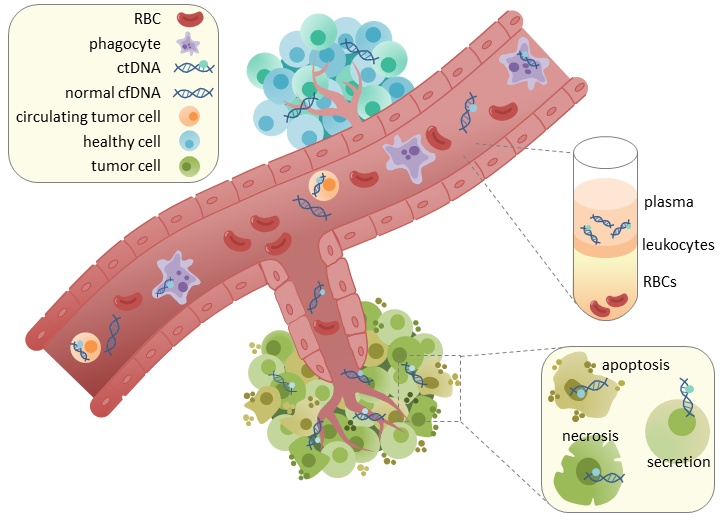
\includegraphics[width=1\textwidth]{images/ctdna.png}
    \caption{Origines des \gls{adnc}. \citeauthor{racheljunewongEnglishCirculatingTumor2017} \cite{racheljunewongEnglishCirculatingTumor2017}.}
    \label{fig:ctdna}
\end{figure}
    
